\documentclass[a4paper,12pt]{report}

% Packages nécessaires
\usepackage[utf8]{inputenc}  % Encodage des caractères
\usepackage[T1]{fontenc}     % Gestion des caractères spéciaux
\usepackage[francais]{babel} % Langue française
\usepackage{graphicx}        % Inclusion des images
\usepackage{hyperref}        % Liens hypertexte
\usepackage{geometry}        % Marges
\geometry{margin=1in}        % Définit des marges de 1 pouce

% images folder
\graphicspath{ {../images/} }

% Informations pour la page de titre
\title{
  
\includegraphics[width=10cm]{../images/logo-univ-evry.png} \\[1cm] % Logo avec chemin vers le fichier
  \textbf{Rapport projet scoring}
}
\author{DIEDHIOU Mamadou, HAOUD Anas, NGETH Laurent, PAZITHNOV Artemii}
\date{\today}

\begin{document}

% Page de titre
\maketitle

% Table des matières
\tableofcontents
\newpage

% Introduction
\chapter{Introduction}
Introduction générale au sujet du rapport. Expliquez le contexte, les objectifs et la structure du document.

% Chapitre 1
\chapter{Les données}
\section{Description des données}
Description détaillée de la première section.

\subsubsection{Variable dépendante (Target)}

En affichant la répartition de la variable "BAD" dans notre dataset (Figure \ref{fig:dis_target}), on voit qu'il y a davantage de cas où les clients ne font pas défauts (BAD = 0)
que de cas où ils font défauts.

\begin{figure}[h!]
  \begin{center}
    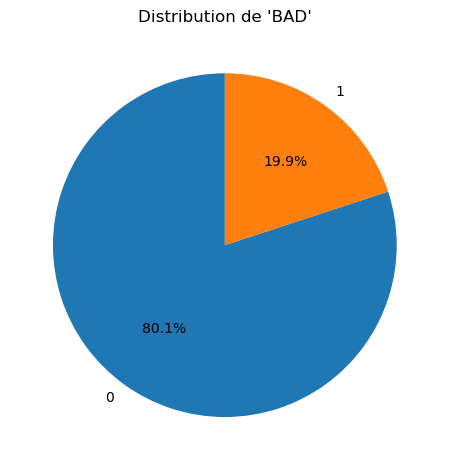
\includegraphics[width=0.5\textwidth]{target_distribution}
  \end{center}
  \caption{Distribution de la variable Target "BAD"}
  \label{fig:dis_target}
\end{figure}

Intuitivement, cela semble tout à fait logique qu'il y ait moins de cas de défaut chez les clients.\\
En effet,

\subsubsection{Variables explicatives}

\section{Visualisation}
Autres détails pertinents pour cette partie.

\subsubsection{Variables numériques}

\textbf{Distribution}

\subsubsection{Variables explicatives}

\textbf{Barplot}

\section{Outliers}

\begin{figure}[h!]
  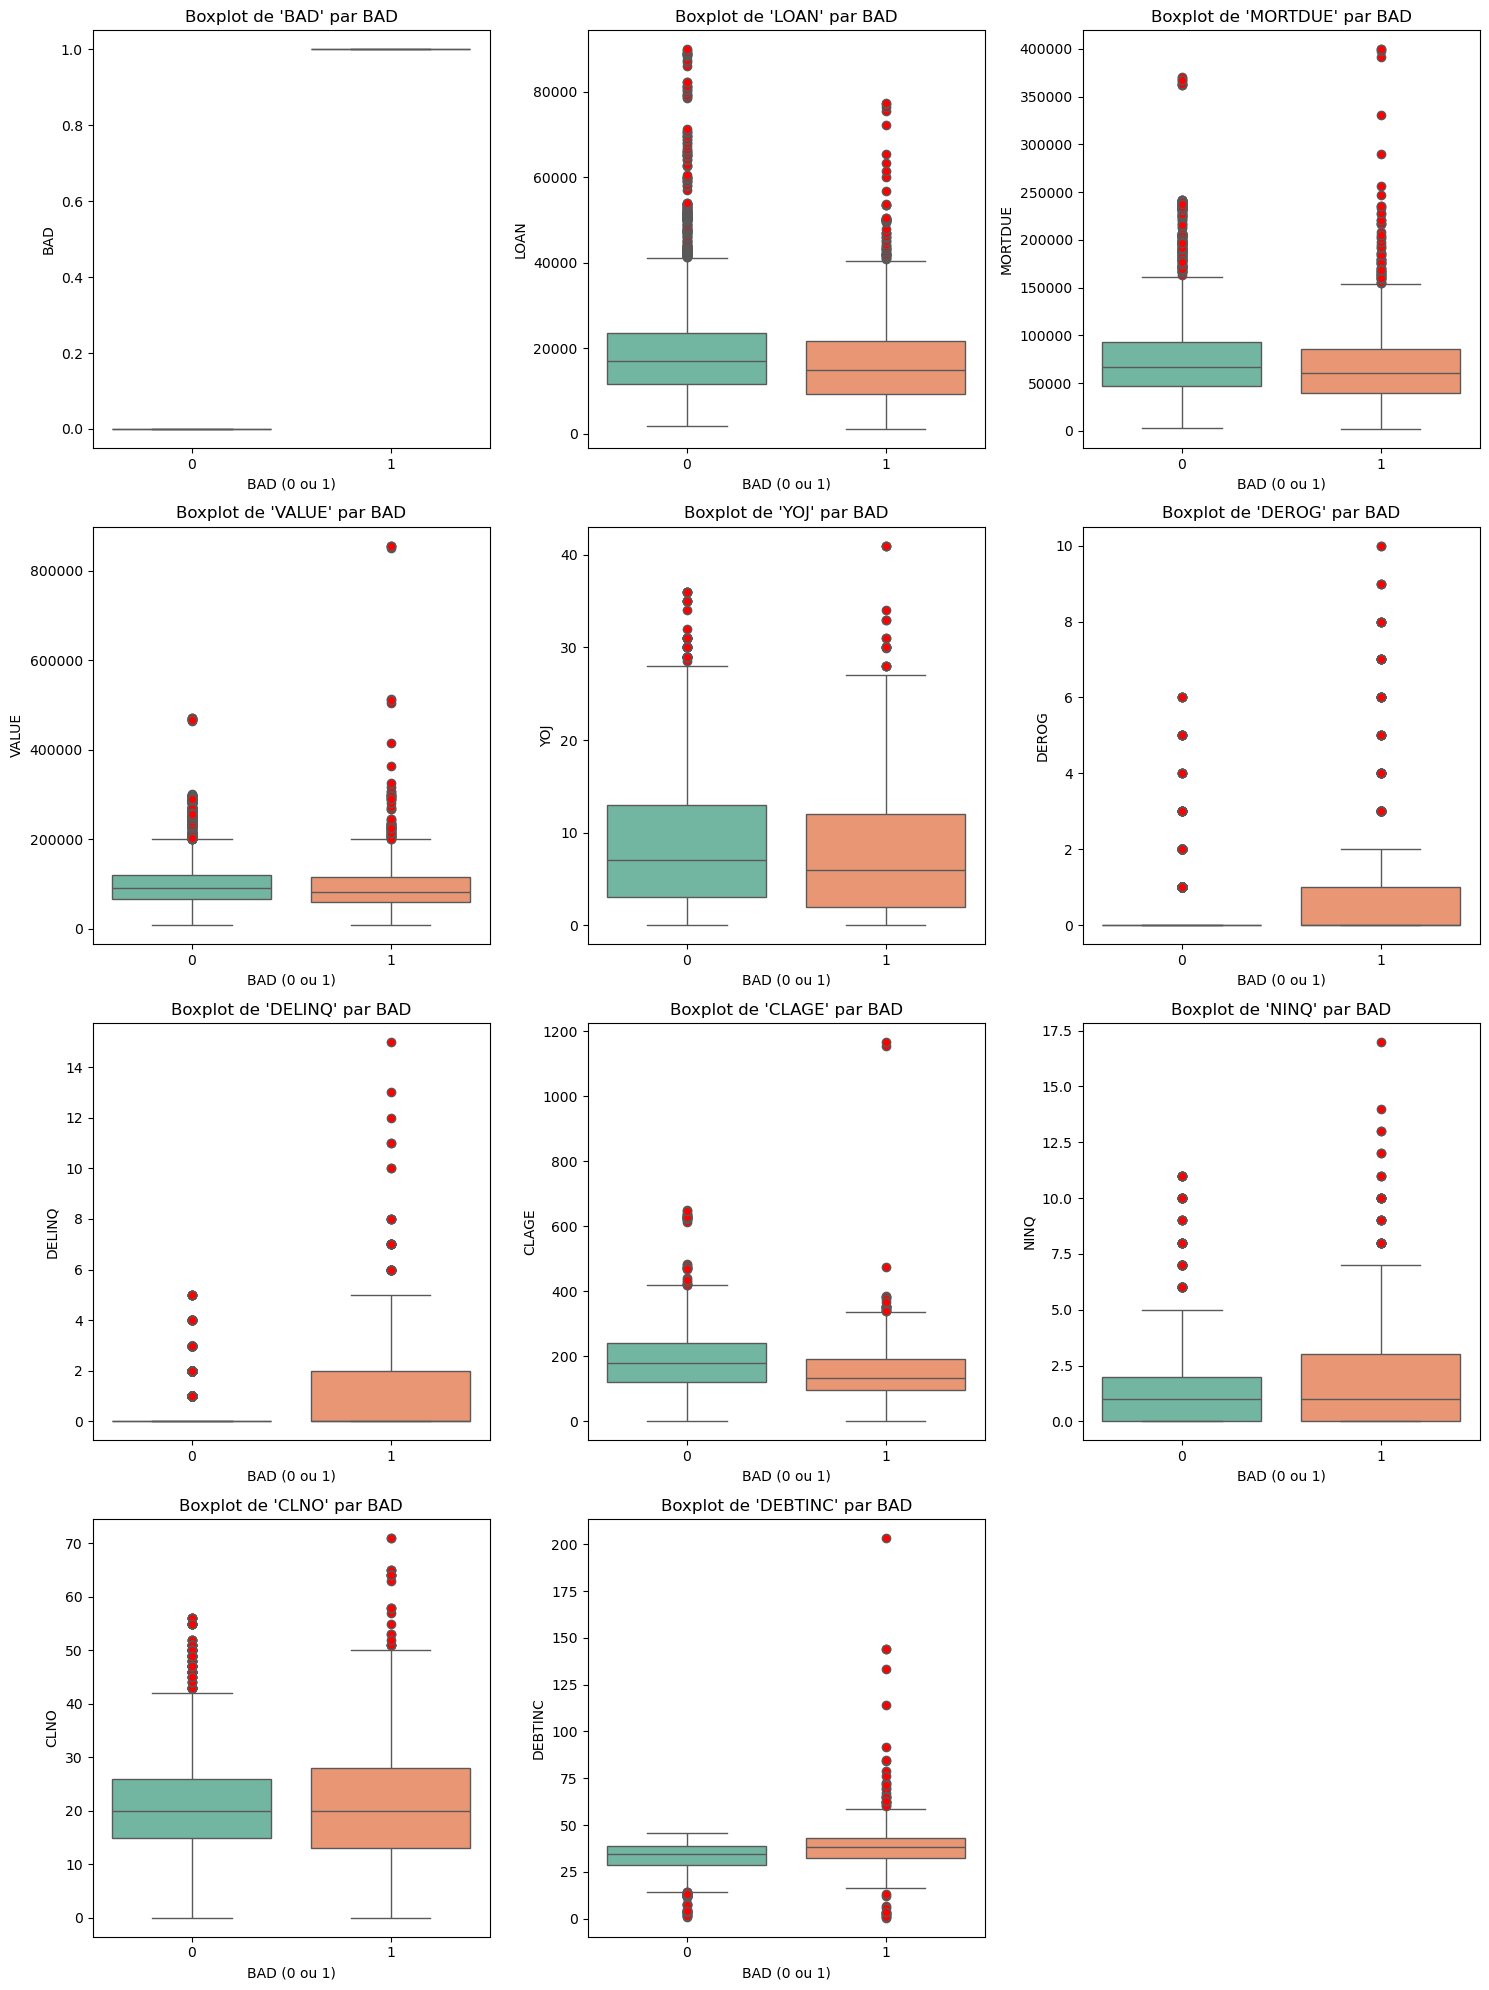
\includegraphics[width=\textwidth]{boxplot_var_num}
  \caption{Boxplot des variables numériques par rapport à BAD}
  \label{fig:boxplot_var_num}
\end{figure}

\section{NaN values}



% Chapitre 2
\chapter{Data processing}

\section{Traitement des valeurs nulles/extrèmes/manquantes}

\subsection{Variables numériques : Imputation par valeur calculée}

Imputation possible :
\begin{itemize}
  \item Par la moyenne --
  \item Par la médiane --
  \item Par KNN --
\end{itemize}

\subsection{Variables catégorielles : Imputation de données}

D'après la répartition des valeurs manquantes dans les variables catégorielles, on voit qu'elles 
uniquement présentes dans "REASON" et "JOB" (Figure \ref{fig:dist_missing_values_cat}).

\begin{figure}[h!]
  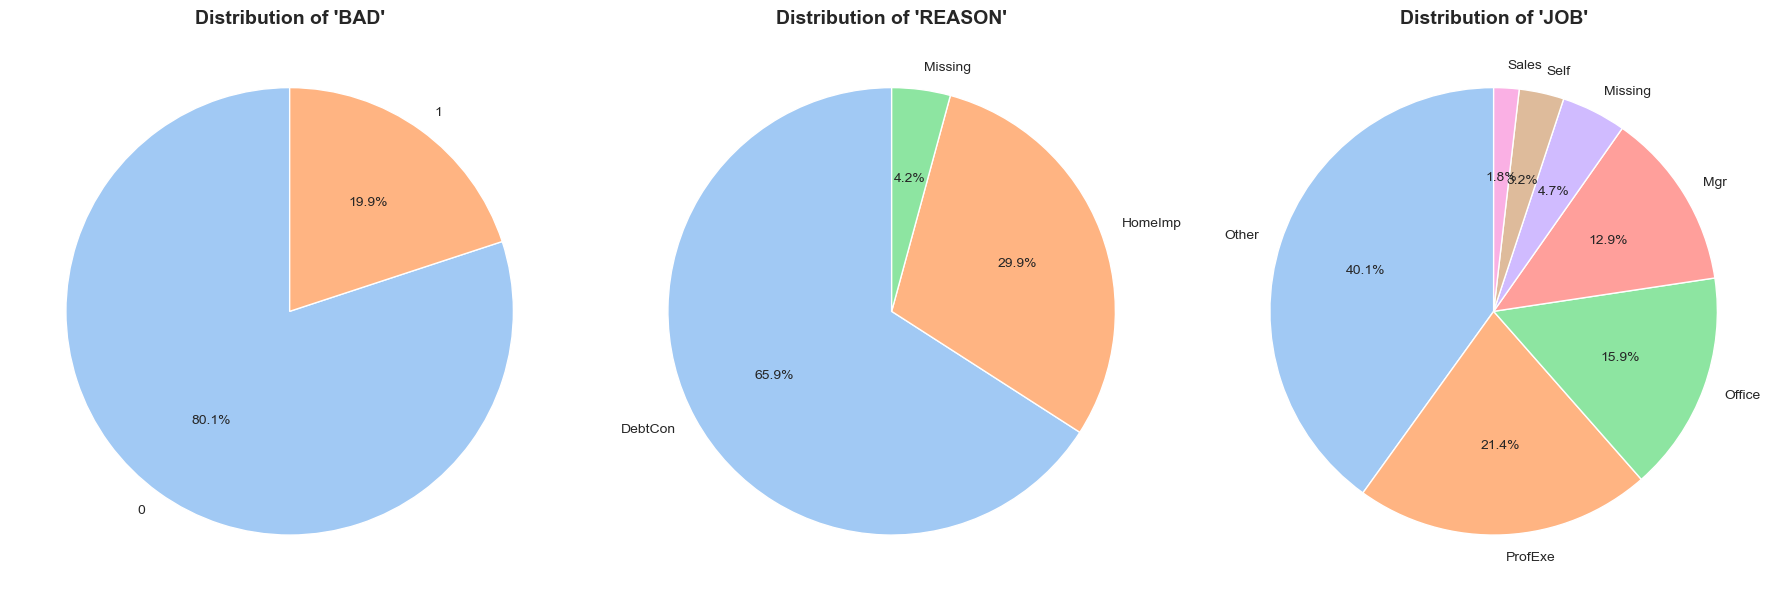
\includegraphics[width=\textwidth]{piechart_valeurs_manquantes_var_categorial}
  \caption{Distribution des valeurs manquantes dans les variables catégorielles}
  \label{fig:dist_missing_values_cat}
\end{figure}

On voit que ces valeurs manquantes représentent aux alentours de 5\% des observations pour les variables "REASON" et "JOB".\\
\\
Nous avons choisi de réaliser une suppression des observations qui possèdent ces 2 variables catégorielles à nulles (Figure \ref{fig:dist_missing_values_cat_dropna}).\\
En effet, pour seulement 5\% des observations, il n'est pas nécessaires de vouloir combler les valeurs manquantes par une interpolation
sachant que cela peut induire davantage de biais dans nos données.\\
Nous avons déjà fait une imputation par KNN pour les valeurs numériques, de ce fait, nous jugeons que cela n'est pas nécessaires vu la quantité de données,
pour les variables catégorielles.
\\

\begin{figure}[h!]
  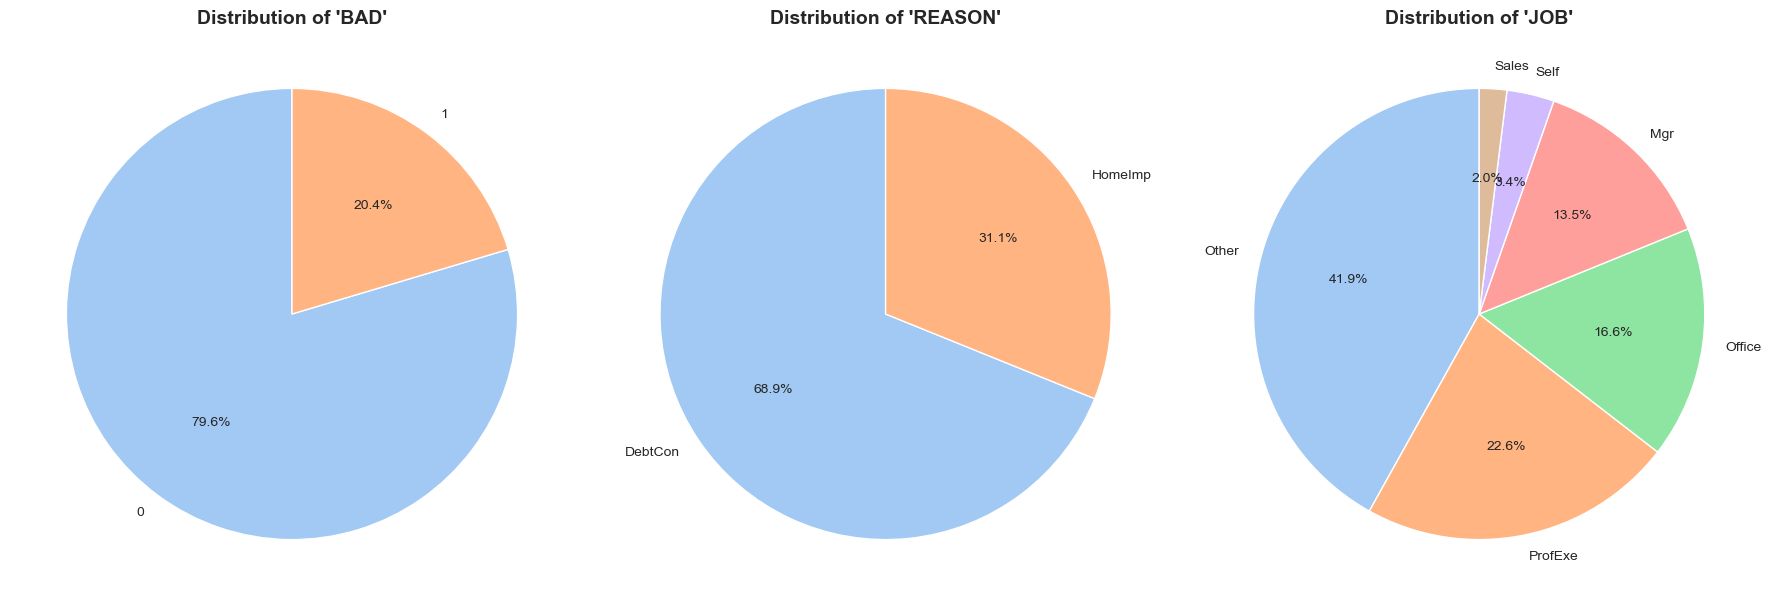
\includegraphics[width=\textwidth]{piechart_valeurs_manquantes_var_categorial_dropna.png}
  \caption{Distribution des valeurs manquantes dans les variables catégorielles après suppression des observations avec NaN}
  \label{fig:dist_missing_values_cat_dropna}
\end{figure}


\chapter{Modélisation}

\section{Sélection des variables}

\subsection{Corrélation entre variable numérique-numérique}

\begin{figure}[h!]
  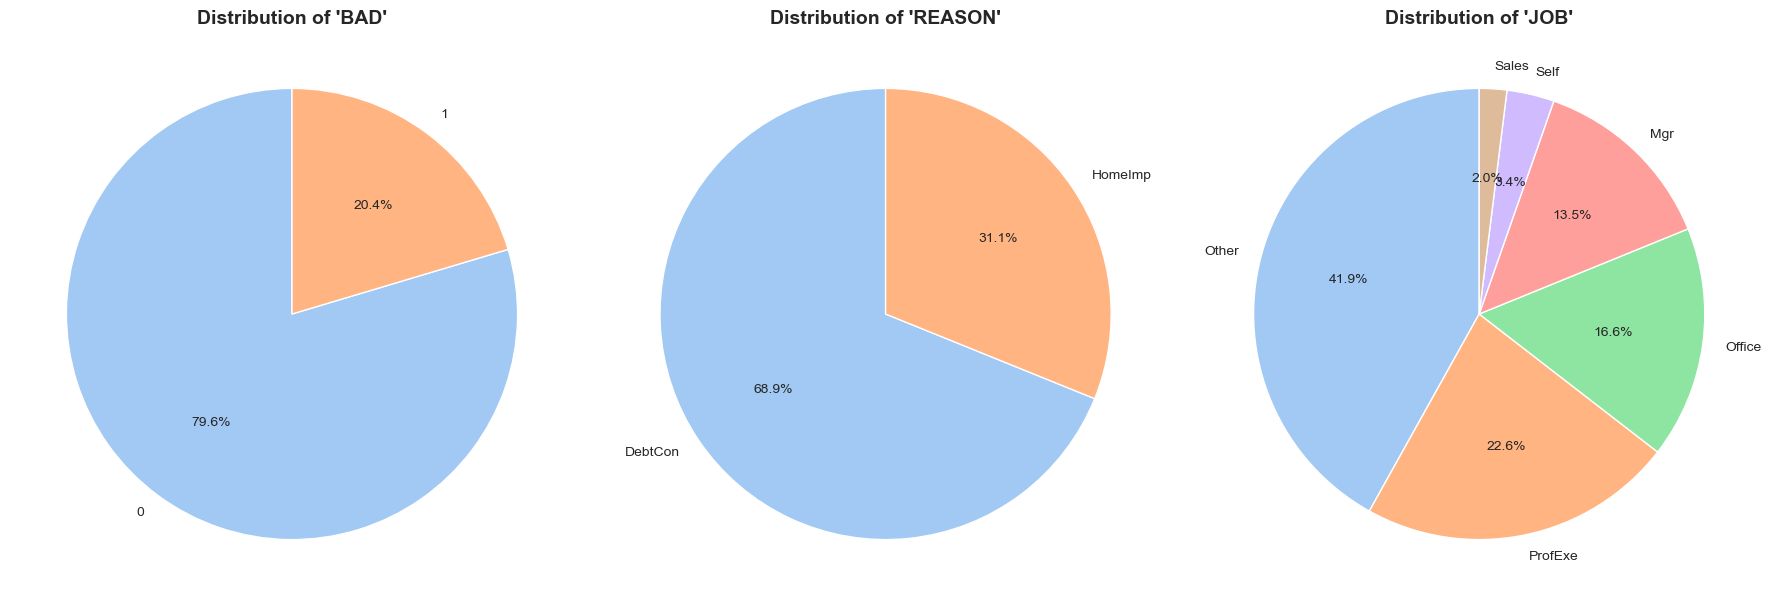
\includegraphics[width=\textwidth]{piechart_valeurs_manquantes_var_categorial_dropna.png}
  \caption{Distribution des valeurs manquantes dans les variables catégorielles après suppression des observations avec NaN}
  \label{fig:}
\end{figure}

\subsection{Corrélation entre variable catégorielle-numérique}
\subsection{Corrélation entre variable catégorielle-catégorielle}


\section{Modèles de classification}

\subsection{Métriques de performances}

Pour mesurer la performances des modèles, on utilse

\subsection{Modèles choisis}

\chapter{Résultats}

% Conclusion
\chapter{Conclusion}
Résumé des points principaux abordés dans le rapport. Incluez les conclusions finales et éventuellement des perspectives pour le futur.

% Bibliographie
\begin{thebibliography}{99}
\bibitem{reference1} Auteur. \emph{Titre du livre ou de l'article}. Maison d'édition, Année.
\bibitem{reference2} Auteur. \emph{Titre du site web}. Consulté le: \today, URL: \url{https://www.example.com}.
\end{thebibliography}

% Annexes
\appendix
\chapter{Annexe A}
Contenu supplémentaire ou données techniques.

\end{document}
